\chapter{Mutation}\label{ch:state}\label{ch:mutation}

\chapquoter{Faced with the choice between changing one's mind and proving that there is no need to do so, almost everyone gets busy on the proof.}{John Kenneth Galbraith}

\begin{schemeregion}

The subset of Scheme we have used until this chapter provides no means to change the value associated with a name.  This enabled very simple evaluation rules for names, as well as allowing the substitution model of evaluation.  Since the value associated with a name was always the value it was defined as, no complex evaluation rules are needed to determine the value associated with a name.  

This chapter introduces special forms known as \definition{mutators} that allow programs to change the value in a given place.  Introducing mutation does not change the computations we can express---every computation that can be expressed using mutation could also be expressed using the only purely functional subset of Scheme from Chapter~\ref{ch:programming}.  It does, however, make it possible to express certain computations more efficiently and clearly than could be done without it.  Adding mutation is not free, however; reasoning about the value of expressions becomes much more complex. 

\section{Assignment}\index{general}{assignment}\index{general}{set!}

The \scheme|set!| (pronounced ``set-bang!'') special form associates a new value with an already defined name.  The exclamation point at the end of \scheme|set!| follows a naming convention to indicate that an operation may mutate state.  A set expression is also known as an \definition{assignment}.  It \emph{assigns} a value to a variable.

The grammar rule for assignment is: 

\begin{bnfgrammarm}{Assignment}
\bnfrule{Expression}{\nonterminal{Assignment}}
\bnfrule{Assignment}{\scheme|(set! \Name \Expression)|}
\end{bnfgrammarm}

The evaluation rule for an assignment is:
\begin{smallquote}
\bold{Evaluation Rule 7: Assignment.}  To evaluate an assignment, evaluate the expression, and replace the value associated with the name with the value of the expression.  An assignment has no value.
\end{smallquote}

Assignments do not produce output values, but are used for their side effects.  They change the value of some state (namely, the value associated with the name in the set expression), but do not produce an output.  \index{general}{side effects}

Here is an example use of \scheme|set!|:
\begin{code}
\scheme|> (define num 200)|\\
\scheme|> num|\\
\schemeresult|200|\\
\scheme|> (set! num 150)|\\
\scheme|> (set! num 1120)|\\
\scheme|> num|\\
\schemeresult|1120|
\end{code}


\shortsection{Begin expression} \index{general}{begin}Since assignments do not evaluate to a value, they are often used inside a begin expression.  A begin expression is a special form that evaluates a sequence of expressions in order and evaluates to the value of the last expression.

The grammar rule for the begin expression is:

\begin{bnfgrammarm}{BeginExpression}
\bnfrule{Expression}{\nonterminal{BeginExpression}}
\bnfrule{BeginExpression}{\scheme|(begin \MoreExpressions \Expression)|}
\end{bnfgrammarm}

The evaluation rule is: 
\begin{smallquote}
\bold{Evaluation Rule 8: Begin.} To evaluate a begin expression, 
\begin{quote}
\scheme|(begin \Expressiona \Expressionb \ldots \Expressionk)|
\end{quote}
evaluate each subexpression in order from left to right. The value of the begin expression is the value of the last subexpression, \scheme|\Expressionk|.
\end{smallquote}
 
The values of all the subexpressions except the last one are ignored; these subexpressions are only evaluated for their side effects.

The begin expression must be a special form. It is not possible to define a procedure that behaves identically to a begin expression since the application rule does not specify the order in which the operand subexpressions are evaluated.  

\index{general}{definition}The definition syntax for procedures includes a hidden begin expression. 
\begin{schemedisplay}
(define (\Name \Parameters) \MoreExpressions \Expression)
\end{schemedisplay}
is an abbreviation for: 
\begin{schemedisplay}
(define \Name
  (lambda (\Parameters) (begin \MoreExpressions \Expression)))
\end{schemedisplay}

The let expression introduced in Section~\ref{sec:best-first-sort} also includes a hidden begin expression. 
\begin{schemedisplay}
(let ((\Namea \Expressiona) (\Nameb \Expressionb)
      \cdots (\Namek \Expressionk))
  \MoreExpressions \Expression)
\end{schemedisplay}
is equivalent to the application expression: 
\begin{schemedisplay}
((lambda (\Namea \Nameb \ldots \Namek)
   (begin \MoreExpressions \Expression))
 \Expressiona \Expressionb \ldots \Expressionk)
\end{schemedisplay}

\section{Impact of Mutation}\label{sec:impactofmutation}

Introducing assignment presents many complications for our programming model.  It invalidates the substitution model of evaluation introduced in Section~\ref{sec:substitution-model} and found satisfactory until this point.  All the procedures we can define without using mutation behave almost like mathematical functions---every time they are applied to the same inputs they produce the same output.\footnote{Observant readers should notice that we have already used a few procedures that are not functions including the printing procedures from Section~\ref{sec:printing}, and \scheme|random| and \scheme|read-char| from the previous chapter.}  Assignments allow us to define non-functional procedures that produce different results for different applications even with the same inputs. 

\begin{examplenobar}{Counter}\label{example:counter} Consider the \scheme|update-counter!| procedure: \index{general}{counter}
\begin{schemedisplay}
(define (update-counter!)
  (set! counter (+ counter 1))
  counter)
\end{schemedisplay}
To use \scheme|update-counter!|, we must first define the \scheme|counter| variable it uses:
\begin{schemedisplay}
(define counter 0)
\end{schemedisplay}
Every time \scheme|(update-counter!)| is evaluated the value associated with the name \scheme|counter| is increased by one and the result is the new value of counter.  Because of the hidden begin expression in the definition, the \scheme|(set! counter (+ counter 1))| is always evaluated first, followed by \scheme|counter| which is the last expression in the begin expression so its value is the value of the procedure.  Thus, the value of \scheme|(update-counter!)| is \schemeresult|1| the first time it is evaluated, \schemeresult|2| the second time, and so on.  

The substitution model of evaluation doesn't make any sense for this evaluation: the value of \scheme|counter| changes during the course of the evaluation.  Even though \scheme|(update-counter!)| is the same expression, every time it is evaluated it evaluates to a different value.\index{general}{substitution}

Mutation also means some expressions have undetermined values.  Consider evaluating the expression \scheme|(+ counter (update-counter!))|.  The evaluation rule for the application expression does not specify the order in which the operand subexpressions are evaluated.  But, the value of the name expression \scheme|counter| depends on whether it is evaluated before or after the application of \scheme|update-counter!| is evaluated!  

The meaning of the expression is ambiguous since it depends on the order in which the subexpressions are evaluated.  If the second subexpression, \scheme|counter|, is evaluated before the third subexpression, \scheme|(update-counter!)|, the value of the expression is \schemeresult|1| the first time it is evaluated, and \schemeresult|3| the second time it is evaluated.  Alternately, but still following the evaluation rules correctly, the third subexpression could be evaluated before the second subexpression.  With this ordering, the value of the expression is \schemeresult|2| the first time it is evaluated, and \schemeresult|4| the second time it is evaluated.    
\end{examplenobar}

\subsection{Names, Places, Frames, and Environments}

Because assignments can change the value associated with a name, the order in which expressions are evaluated now matters.  As a result, we need to revisit several of our other evaluation rules and change the way we think about processes. 

Since the value associated with a name can now change, instead of associating a value directly with a name we use a name as a way to identify a \definition{place}.  A place has a name and holds the value associated with that name.  With mutation, we can change the value in a place; this changes the value associated with the place's name.  A \definition{frame} is a collection of places.

An \definition{environment} is a pair consisting of a frame and a pointer to a parent environment.  A special environment known as the \emph{global environment}\index{general}{global environment} has no parent environment.  The global environment exists when the interpreter starts, and is maintained for the lifetime of the interpreter.  Initially, the global environment contains the built-in procedures.  Names defined in the interactions buffer are placed in the global environment.  Other environments are created and destroyed as a program is evaluated.  Figure~\ref{fig:environment} shows some example environments, frames, and places.

\begin{figure}[!b]
\begin{center}
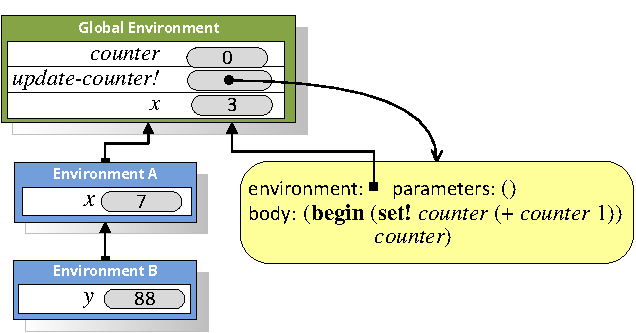
\includegraphics[width=4.8in]{figures/environment.pdf}
\caption{Sample environments.}\label{fig:environment}
\subcapw{The global environment contains a frame with three names.  Each name has an associated place that contains the value associated with that name.  The value associated with \scheme|counter| is the currently \schemeresult|0|.  The value associated with \scheme|set-counter!| is the procedure we defined in Example~\ref{example:counter}.  A procedure is characterized by its parameters, body code, and a pointer to the environment in which it will be evaluated.}
\end{center}
\end{figure}

Every environment has a parent environment except for the global environment.  All other environments descend from the global environment.  Hence, if we start with any environment, and continue to follow its parent pointers we always eventually reach the global environment.

The key change to our evaluation model is that whereas before we could evaluate expressions without any notion of \emph{where} they are evaluated, once we introduce mutation, we need to consider the environment in which an expression is evaluated.  An environment captures the current state of the interpreter.  The value of an expression depends on both the expression itself, and on the environment in which it is evaluated.

\subsection{Evaluation Rules with State}\label{sec:state-rules}

Introducing mutation requires us to revise the evaluation rule for names, the definition rule, and the application rule for constructed procedures.  All of these rules must be adapted to be more precise about how values are associated with names by using places and environments.

\shortsection{Names} The new evaluation rule for a name expression is:

\mevalrule{Stateful Evaluation Rule 2: Names}{To evaluate a name expression, search the evaluation environment's frame for a place with a name that matches the name in the expression.  If such a place exists, the value of the name expression is the value in that place.  Otherwise, the value of the name expression is the result of evaluating the name expression in the parent environment.  If the evaluation environment has no parent, the name is not defined and the name expression evaluates to an error.}

For example, to evaluate the value of the name expression \scheme|x| in Environment B in Figure~\ref{fig:environment}, we first look in the frame of Environment B for a place named \scheme|x|.  Since there is no place named \scheme|x| in that frame, we follow the parent pointer to Environment A, and evaluate the value of the name expression in Environment A.  Environment A's frame contains a place named \scheme|x| that contains the value \schemeresult|7|, so the value of evaluating \scheme|x| in Environment B is \schemeresult|7|.  

The value of the same expression in the Global Environment is \schemeresult|3| since that is the value in the place named \scheme|x| in the Global Environment's frame.  

To evaluate the value of \scheme|y| in Environment A, we first look in the frame in Environment A for a place named \scheme|y|.  Since no \scheme|y| place exists, evaluation continues by evaluating the expression in the parent environment, which is the Global Environment.  The Global Environment�s frame does not contain a place named \scheme|y|, and the global environment has no parent, so the name is undefined and the evaluation results in an error.

\shortsection{Definition} The revised evaluation rule for a definition is:

\mevalrule{Stateful Definition Rule}{A definition creates a new place with the definition's name in the frame associated with the evaluation environment.  The value in the place is value of the definition's expression.  If there is already a place with the name in the current frame, the definition replaces the old place with a new place and value.}

The rule for redefinitions means we could use \scheme|define| in some situations to mean something similar to \scheme|set!|.  The meaning is different, though, since an assignment finds the place associated with the name and puts a new value in that place.  Evaluating an assignment follows the Stateful Evaluation Rule 2 to find the place associated with a name.  Hence, \scheme|(define \Name \Expression)| has a different meaning from \scheme|(set! \Name \Expression)| when there is no place named \emph{Name} in the current execution environment.  To avoid this confusion, only use \scheme|define| for the first definition of a name and always use \scheme|set!| when the intent is to change the value associated with a name.

\shortsection{Application} The final rule that must change because of mutation is the application rule for constructed procedures.  Instead of using substitution, the new application rule creates a new environment with a frame containing places named for the parameters.  

\mevalrule{Stateful Application Rule 2: Constructed Procedures}{To apply a constructed procedure:
\begin{enumtight}
\item Construct a new environment, whose parent is the environment of the applied procedure.
\item For each procedure parameter, create a place in the frame of the new environment with the name of the parameter.  Evaluate each operand expression in the environment or the application and initialize the value in each place to the value of the corresponding operand expression.
\item Evaluate the body of the procedure in the newly created environment.  The resulting value is the value of the application.
\end{enumtight}}

Consider evaluating the application expression \scheme|(bigger 3 4)| where \scheme|bigger| is the procedure from Example~\ref{example:bigger}: \scheme|(define (bigger a b) (if (> a b) a b)))|.

Evaluating an application of \scheme|bigger| involves following the Stateful Application Rule 2.  First, create a new environment.  Since \scheme|bigger| was defined in the global environment, its environment pointer points to the global environment.  Hence, the parent environment for the new environment is the global environment.  

Next, create places in the new environment's frame named for the procedure parameters, \scheme|a| and \scheme|b|.  The value in the place associated with \scheme|a| is \schemeresult|3|, the value of the first operand expression.  The value in the place associated with \scheme|b| is \schemeresult|4|.  

The final step is to evaluate the body expression, \scheme|(if (> a b) a b)|, in the newly created environment.  Figure~\ref{fig:evalmax} shows the environment where the body expression is evaluated.  The values of \scheme|a| and \scheme|b| are found in the application environment.

\begin{figure}[bht]
\begin{center}
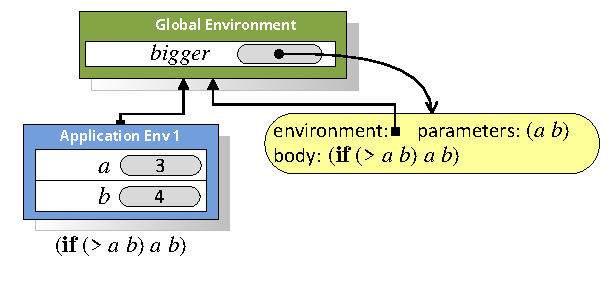
\includegraphics[width=4.5in]{figures/evalmax.pdf}
\caption{Environment created to evaluate (\var{bigger} \snumber{3} \snumber{4}).}\label{fig:evalmax}\LATER{make it look like scheme mode}
\end{center}
\end{figure}

The new application rule becomes more interesting when we consider procedures that create new procedures.  For example, \scheme|make-adder| takes a number as input and produces as output a procedure:
\begin{schemedisplay}
(define (make-adder v) (lambda (n) (+ n v)))
\end{schemedisplay}

The environment that results from evaluating \scheme|(define inc (make-adder 1))| is shown in Figure~\ref{fig:make-adder}.  The name \scheme|inc| has a value that is the procedure resulting from the application of \scheme|(make-adder 1)|.  To evaluate the application, we follow the application rule above and create a new environment containing a frame with the parameter name, \scheme|inc|, and its associated operand value, \schemeresult|1|.  

\begin{figure}[bth]
\begin{center}
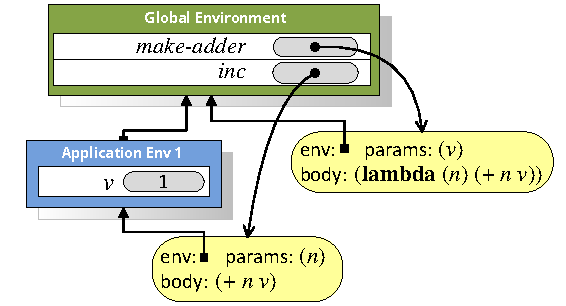
\includegraphics[width=4.5in]{figures/eval-make-adder.pdf}
\caption{Environment after evaluating (\bold{define} \var{inc} (\var{make-adder} \snumber{1})).}\label{fig:make-adder}\LATER{Fix scheme}
\end{center}
\end{figure}

The result of the application is the value of evaluating its body in this new environment.  Since the body is a lambda expression, it evaluates to a procedure.  That procedure was created in the execution environment that was created to evaluate the application of \scheme|make-adder|, hence, its environment pointer points to the application environment which contains a place named \scheme|inc| holding the value \schemeresult|1|.

Next, consider evaluating \scheme|(inc 149)|.  Figure~\ref{fig:inc-app} illustrates the environment for evaluating the body of the \scheme|inc| procedure.  The evaluation creates a new environment with a frame containing the place \scheme|n| and its associated value \schemeresult|149|.  We evaluate the body of the procedure, \scheme|(+ n v)|, in that environment.  The value of \scheme|n| is found in the execution environment.  The value of \scheme|v| is not found there, so evaluation continues by looking in the parent environment.  It contains a place \scheme|v| containing the value \schemeresult|1|.

\begin{figure}[bht]
\begin{center}
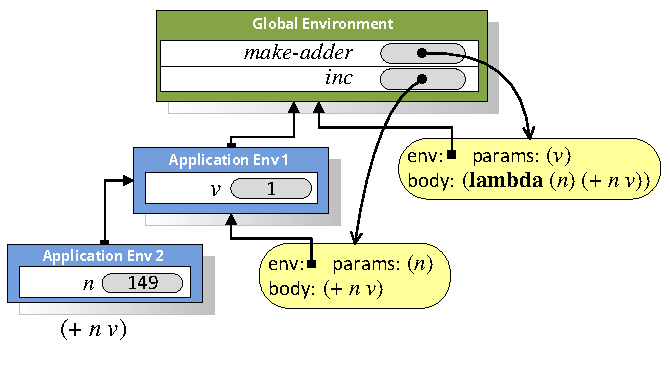
\includegraphics[width=4.5in]{figures/eval-apply-inc.pdf}
\caption{Environment for evaluating the body of (\var{inc} \snumber{149}).\label{fig:inc-app}}\LATER{FIX!}
\end{center}
\end{figure}

\beforeex
\begin{exercise}\greenstar
Devise a Scheme expression that could have four possible values, depending on the order in which application subexpressions are evaluated.
\solution{\LATER{}}
\end{exercise}
\afterex

\beforeex
\begin{exercise}
Draw the environment that results after evaluating:
\begin{code}
\scheme|> (define alpha 0)|\\
\scheme|> (define beta 1)|\\
\scheme|> (define update-beta! (lambda () (set! beta (+ alpha 1)))|\\
\scheme|> (set! alpha 3)|\\
\scheme|> (update-beta!)|\\
\scheme|> (set! alpha 4)|\\
\end{code}
\solution{\LATER{}}
\end{exercise}
\afterex

\beforeex
\begin{exercise}
Draw the environment that results after evaluating the following expressions, and explain what the value of the final expression is.  (Hint: first, rewrite the let expression as an application.)
\begin{code}
\scheme|> (define (make-applier proc) (lambda (x) (proc x))|\\
\scheme|> (define p (make-applier (lambda (x) (let ((x 2)) x))))|\\
\scheme|> (p 4)|\\
\end{code}
\solution{\LATER{}}
\end{exercise}
\afterex

\section{Mutable Pairs and Lists}\label{sec:mutablepairs}\index{general}{set-mcar!}\index{general}{set-mcdr!}\index{general}{mutable pair}\index{general}{mcons}

The Pair datatype introduced in Chapter~\ref{ch:data} is \definition{immutable}.  This means that once a Pair is created, the values in its cells cannot be changed.\footnote{The mutability of standard Pairs is quite a controversial issue.  In most Scheme implementations and the standard definition of Scheme, a standard \scheme|cons| pair is mutable.  But, as we will see later in the section, mutable pairs cause lots of problems.  So, the designers of DrRacket decided for Version 4.0 to make the standard Pair datatype immutable and to provide a MutablePair datatype for use when mutation is needed.}  

The MutablePair datatype is a mutable pair.  A MutablePair is constructed using \scheme|mcons|, which is similar to \scheme|cons| but produces a MutablePair.  The parts of a MutablePair can be extracted using the \scheme|mcar| and \scheme|mcdr| procedures, which behave analogously to the \scheme|car| and \scheme|cdr| procedures.  A MutablePair is a distinct datatype from a Pair; it is an error to apply \scheme|car| to a MutablePair, or to apply \scheme|mcar| to an immutable Pair.

The MutablePair datatype also provides two procedures that change the values in the cells of a MutablePair:
\begin{descriptionlist}
\item [\scheme|set-mcar!|: MutablePair $\times$ Value $\rightarrow$ Void] \forcenl Replaces the value in the first cell of the MutablePair with the value of the second input.  
\item [\scheme|set-mcdr!|: MutablePair $\times$ Value $\rightarrow$ Void] \forcenl Replaces the value in the second cell of the MutablePair with the value of the second input.  
\end{descriptionlist}
The Void result type indicates that \scheme|set-mcar!| and \scheme|set-mcdr!| produce no output.

Here are some interactions using a MutablePair:
\begin{code}
\scheme|> (define pair (mcons 1 2))|\\
\scheme|> (set-mcar! pair 3)|\\
\scheme|> pair|\\
\schemeresult|(3 . 2)|\\
\scheme|> (set-mcdr! pair 4)|\\
\scheme|> pair|\\
\schemeresult|(3 . 4)|
\end{code}
The \scheme|set-mcdr!| procedure allows us to create a pair where the second cell of the pair is itself: \scheme|(set-mcdr! pair pair)|.  This produces the rather frightening object shown in Figure~\ref{fig:circular-pair}.  
\begin{figure}[!tbh]\centering
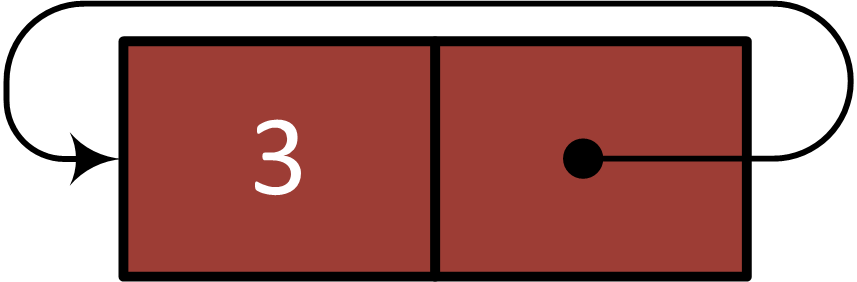
\includegraphics{figures/circular-pair.png}
\caption{Mutable pair created by evaluating (\var{set-mcdr!} \var{pair} \var{pair}).\label{fig:circular-pair}}
\end{figure}
Every time we apply \scheme|mcdr| to \scheme|pair|, we get the same pair as the output.  Hence, the value of \scheme|(mcar (mcdr (mcdr (mcdr pair))))| is \schemeresult|3|.

We can also create objects that combine mutable and immutable Pairs.  For example, \scheme|(define mstruct (cons (mcons 1 2) 3))| defines \scheme|mstruct| as an immutable Pair containing a MutablePair in its first cell.  Since the outer Pair is immutable, we cannot change the objects in its cells.  Thus, the second cell of \scheme|mstruct| always contains the value \snumber{3}.  We can, however, change the values in the cells of the mutable pair in its first cell.  For example, \scheme|(set-mcar! (car mstruct) 7)| replaces the value in the first cell of the MutablePair in the first cell of \scheme|mstruct|.

\index{general}{mutable lists}\index{general}{mlist}
\shortsection{Mutable Lists} As we used immutable Pairs to build immutable Lists, we can use MutablePairs to construct MutableLists.  A MutableList is either \schemeresult|null| or a MutablePair whose second cell contains a MutableList.  

The MutableList type is defined by a library.  To use it, evaluate the following expression: \scheme|(require racket/mpair)|.  All of the examples in this chapter assume this expression has been evaluated.  This library defines the \scheme|mlist| procedure that is similar to the \scheme|list| procedure, but produces a MutableList instead of an immutable List.  For example, \scheme|(mlist 1 2 3)| produces the structure shown in Figure~\ref{fig:mlist}.  
\begin{figure}[bthp]\centering

\includegraphics{figures/mlist.png}
\caption{MutableList created by evaluating (\var{mlist} \snumber{1} \snumber{2} \snumber{3}).\label{fig:mlist}}\LATER{FIX}
\end{figure}
Each node in the list is a MutablePair, so we can use the \scheme|set-mcar!| and \scheme|set-mcdr!| procedures to change the values in the cells.
\begin{code}
\scheme|> (define m1 (mlist 1 2 3))|\\
\scheme|> (set-mcar! (mcdr m1) 5)|\\
\scheme|> (set-mcar! (mcdr (mcdr m1)) 0)|\\
\scheme|> m1|\\
\schemeresult|{1 5 0}| \emph{; DrRacket denotes MutableLists using curly brackets.}
\end{code}
Many of the list procedures from Chapter~\ref{ch:data} can be directly translated to work on mutable lists.  For example, we can define \scheme|mlist-length| as:
\begin{schemedisplay}
(define (mlist-length m)
  (if (null? m) 0 (+ 1 (mlist-length (mcdr m)))))
\end{schemedisplay}
As shown in Exercise~\ref{exercise:mlist}, though, we need to be careful when using \scheme|mcdr| to recurse through a MutableList since structures created with MutablePairs can include circular pointers.

\beforeex
\begin{exercise}\label{exercise:mlist} 
What is the value of \scheme|(mlist-length pair)| for the pair shown in Figure~\ref{fig:circular-pair}?
\solution{\LATER{}}
\end{exercise}
\afterex

\beforeex
\begin{exercise}\goldstar
Define a \scheme|mpair-circular?| procedure that takes a MutablePair as its input and outputs \schemeresult|true| when the input contains a cycle and \schemeresult|false| otherwise.
% \scheme|mpair-circular?| is applied to any MutablePair for which repeated \scheme|mcdr| operations will never reach \scheme|null|.
\solution{\LATER{}}
\end{exercise}
\afterex

\section{Imperative Programming}\index{general}{imperative programming}\index{general}{functional programming}

Mutation enables a style of programming known as \definition{imperative programming}.  Whereas \emph{functional programming} is concerned with defining procedures that can be composed to solve a problem, imperative programming is primarily concerned with modifying state in ways that lead to a state that provides a solution to a problem.  

The main operation in function programming is application.  A functional program applies a series of procedures, passing the outputs of one application as the inputs to the next procedure application.  With imperative programming, the primary operation is assignment (performed by \scheme|set!|, \scheme|set-mcar!|, and \scheme|set-mcdr!| in Scheme; but typically by an assignment operator, often \verb|:=| or \verb|=|, in languages designed for imperative programming such as Pascal, Algol60, Java, and Python).   

The next subsection presents imperative-style versions of some of the procedures we have seen in previous chapters for manipulating lists.  The following subsection introduces some imperative control structures.

\subsection{List Mutators}

All the procedures for changing the value of a list in Section~\ref{sec:constructing-lists} actually do not change any values; instead they construct new lists.  When our goal is only to change some elements in an existing list, this wastes memory constructing a new list and may require more running time than a procedure that modifies the input list instead.  Here, we revisit some of the procedures from Section~\ref{sec:constructing-lists}, but instead of producing new lists with the desired property these procedures modify the input list.

\begin{examplenobar}{Mapping} The \scheme|list-map| procedure (from Example~\ref{example:map}) produces a new list that is the result of applying the same procedure to every element in the input list.  
\begin{schemedisplay}
(define (list-map f p)
  (if (null? p) null (cons (f (car p)) (list-map f (cdr p)))))
\end{schemedisplay} 
Whereas the functional \scheme|list-map| procedure uses \scheme|cons| to build up the output list, the imperative \scheme|mlist-map!| procedure uses \scheme|set-car!| to mutate the input list's elements:
\begin{schemedisplay}
(define (mlist-map! f p)
  (if (null? p) (void)
      (begin (set-mcar! p (f (mcar p)))
             (mlist-map! f (mcdr p)))))
\end{schemedisplay}
The base case uses \scheme|(void)| to evaluate to no value.  Unlike \scheme|list-map| which evaluates to a List, \scheme|mlist-map!| is evaluated for its side effects and produces no output.

Assuming the procedure passed as \scheme|f| has constant running time, the running time of the \scheme|mlist-map!| procedure is in $\Theta(n)$ where $n$ is the number of elements in the input list.  There will be $n$ recursive applications of \scheme|mlist-map!| since each one passes in a list one element shorter than the input list, and each application requires constant time.  This is asymptotically the same as the \scheme|list-map| procedure, but we would expect the actual running time to be faster since there is no need to construct a new list.  

The memory consumed is asymptotically different.  The \scheme|list-map| procedure allocates $n$ new \scheme|cons| cells, so it requires memory in $\Theta(n)$ where $n$ is the number of elements in the input list.  The \scheme|mlist-map!| procedure is tail recursive (so no stack needs to be maintained) and does not allocate any new \scheme|cons| cells, so it requires constant memory.
\end{examplenobar}

\begin{examplenobar}{Filtering} The \scheme|list-filter| procedure takes as inputs a test procedure and a list and outputs a list containing the elements of the input list for which applying the test procedure evaluates to a true value.  In Example~\ref{example:filter}, we defined \scheme|list-filter| as:
\begin{schemedisplay}
(define (list-filter test p)
   (if (null? p) null
       (if (test (car p)) (cons (car p) (list-filter test (cdr p)))
           (list-filter test (cdr p)))))
\end{schemedisplay}

An imperative version of \scheme|list-filter| removes the unsatisfying elements from a mutable list.  We define \scheme|mlist-filter!| using \scheme|set-mcdr!| to skip over elements that should not be included in the filtered list:
\begin{schemedisplay}
(define (mlist-filter! test p)
  (if (null? p) null
      (begin (set-mcdr! p (mlist-filter! test (mcdr p)))
             (if (test (mcar p)) p (mcdr p)))))
\end{schemedisplay}

Assuming the test procedure has constant running time, the running time of the \scheme|mlist-filter!| procedure is linear in the length of the input list.  As with \scheme|mlist-map!|, the space used by \scheme|mlist-filter!| is constant, which is better than the $\Theta(n)$ space used by \scheme|list-filter|.

Unlike \scheme|mlist-map!|, \scheme|mlist-filter!| outputs a value.  This is needed when the first element is not in the list.  Consider this example:
\begin{code}
\scheme|> (define a (mlist 1 2 3 1 4))|\\
\scheme|> (mlist-filter! (lambda (x) (> x 1)) a)|\\
\schemeresult|{2 3 4}|\\
\scheme|> a|\\
\schemeresult|{1 2 3 4}|
\end{code}
The value of \scheme|a| still includes the initial \schemeresult|1|.  There is no way for the \scheme|mlist-filter!| procedure to remove the first element of the list: the \scheme|set-mcar!| and \scheme|set-mcdr!| procedures only enable us to change what the mutable pair's components contain.  

To avoid this, \scheme|mlist-filter!| should be used with \scheme|set!| to assign the variable to the resulting mutable list: 
\begin{schemedisplay}
(set! a (mlist-filter! (lambda (x) (> x 1)) a))
\end{schemedisplay}
\end{examplenobar}

\begin{example}{Append} \index{general}{list-append}\index{general}{mlist-append!}The \scheme|list-append| procedure takes as input two lists and produces a list consisting of the elements of the first list followed by the elements of the second list.  An imperative version of this procedure instead mutates the first list to contain the elements of both lists.
\begin{schemedisplay}
(define (mlist-append! p q)
  (if (null? p) (error "Cannot append to an empty list")
      (if (null? (mcdr p)) (set-mcdr! p q)
          (mlist-append! (mcdr p) q))))
\end{schemedisplay}
The \scheme|mlist-append!| procedure produces an error when the first input is \scheme|null| --- this is necessary since if the input is \scheme|null| there is no pair to modify.\footnote{The \scheme|mappend!| library procedure in DrRacket takes a different approach: when the first input is null it produces the value of the second list as output in this case.  This has unexpected behavior when an expression like \scheme|(append! a b)| is evaluated where the value of \scheme|a| is \scheme|null| since the value of \scheme|a| is not modified.}

Like \scheme|list-append|, the running time of the \scheme|mlist-append!| procedure is in $\Theta(n)$ where $n$ is the number of elements in the first input list.  The \scheme|list-append| procedure copies the first input list, so its memory use is in $\Theta(n)$ where $n$ is the number of elements in the first input list.  The memory use of \scheme|mlist-append!| is constant: it does not create any new cons cells to append the lists.
\end{example}

\shortsection{Aliasing}\index{general}{aliasing}  Adding mutation makes it possible to define many procedures more efficiently and compactly, but introduces many new potential pitfalls in producing reliable programs.  Since our evaluation model now depends on the environment in which an expression is evaluated, it becomes much harder to reason about code by itself. 

One challenge introduced by mutation is \definition{aliasing}.  There may be different ways to refer to the same object.  This was true before mutation also, but didn't matter since the value of an object never changed.  Once object values can change, however, aliasing can lead to surprising behaviors.  

For example,
\begin{code}
\scheme|> (define m1 (mlist 1 2 3))|\\
\scheme|> (define m2 (mlist 4 5 6))|\\
\scheme|> (mlist-append! m1 m2)|\\
%\scheme|> m1|\\
%\schemeresult|{1 2 3 4 5 6}|\\
%\scheme|> m2|\\
%\schemeresult|{4 5 6}|\\
\scheme|> (set! m1 (mlist-filter! (lambda (el) (= (modulo el 2) 0)) m1))|\\
%\scheme|> m1|\\
%\schemeresult|{2 4 6}|
\end{code}
The value of \scheme|m2| was defined as \schemeresult|{4 5 6}|, and no expressions since then explicitly modified \scheme|m2|.  But, the value of \scheme|m2| has still changed!  It changed because after evaluating \scheme|(mlist-append! m1 m2)| the \scheme|m1| object shares cells with \scheme|m2|.  Thus, when the \scheme|mlist-filter!| application changes the value of \scheme|m1|, it also changes the value of \scheme|m2| to \schemeresult|{4 6}|.

\index{general}{eq?}The built-in procedure \scheme|eq?| takes as input any two objects and outputs a Boolean.  The result is \schemeresult|true| if and only if the inputs are the same object.  For example, \scheme|(eq? 3 3)| evaluates to \schemeresult|true| but \scheme|(eq? (mcons 1 2) (mcons 1 2))| evaluates to \schemeresult|false|.  Even though the input pairs have the same value, they are different objects---mutating one of the pairs does not effect the value of the other pair. 

For the earlier \scheme|mlist-append!| example, \scheme|(eq? m1 m2)| evaluates to \schemeresult|false| since \scheme|m1| and \scheme|m2| do not refer to the same object.  But, \scheme|(eq? (mcdr m1) m2)| evaluates to \schemeresult|true| since the second cell of \scheme|m1| points to the same object as \scheme|m2|.  Evaluating \scheme|(set-mcar! m2 3)| changes the value of both \scheme|m1| and \scheme|m2| since the modified cell is common to both structures.

\beforeex
\begin{exercise}
Define an imperative-style procedure, \scheme|mlist-inc!| that takes as input a MutableList of Numbers and modifies the list by adding one to the value of each element in the list.
\solution{\LATER{}}
\end{exercise}
\afterex

\beforeex
\begin{exercise}\goldstar 
Define a procedure \scheme|mlist-truncate!| that takes as input a MutableList and modifies the list by removing the last element in the list.  Specify carefully the requirements for the input list to your procedure.
\solution{\LATER{}}
\end{exercise}
\afterex

\beforeex
\begin{exercise}\goldstar 
Define a procedure \scheme|mlist-make-circular!| that takes as input a MutableList and modifies the list to be a circular list containing all the elements in the original list.  For example, \scheme|(mlist-make-circular! (mlist 3))| should produce the same structure as the circular pair shown in Figure~\ref{fig:circular-pair}.
\solution{\LATER{}}
\end{exercise}
\afterex

\sidequote{If you steal property, you must report its fair market value in your income in the year you steal it unless in the same year, you return it to its rightful owner.}{\emph{Your Federal Income Tax}, IRS Publication 17, 2009.}

\beforeex
\begin{exercise}\goldstar
Define an imperative-style procedure, \scheme|mlist-reverse!|, that reverses the elements of a list.  Is it possible to implement a \scheme|mlist-reverse!| procedure that is asymptotically faster than the \scheme|list-reverse| procedure from Example~\ref{example:map}?
\solution{\LATER{}}
\end{exercise}
\afterex

\beforeex
\begin{exercise}\doublegoldstar 
Define a procedure \scheme|mlist-aliases?| that takes as input two mutable lists and outputs \schemeresult|true| if and only if there are any mcons cells shared between the two lists.
\solution{\LATER{}}
\end{exercise}
\afterex

\subsection{Imperative Control Structures}

The imperative style of programming makes progress by using assignments to manipulate state.  In many cases, solving a problem requires repeated operations.  With functional programming, this is done using recursive definitions.  We make progress towards a base case by passing in different values for the operands with each recursive application.  With imperative programming, we can make progress by changing state repeatedly without needing to pass in different operands. 

A common control structure in imperative programming is a \definition{while loop}.  A while loop has a test condition and a body.  The test condition is a predicate.  If it evaluates to true, the while loop body is executed.  Then, the test condition is evaluated again.  The while loop continues to execute until the test condition evaluates to false.  

We can define \scheme|while| as a procedure that takes as input two procedures, a test procedure and a body procedure, each of which take no parameters.  Even though the test and body procedures take no parameters, they need to be procedures instead of expressions, since every iteration of the loop should re-evaluate the test and body expressions of the passed procedures. 
\begin{schemedisplay}
(define (while test body)
  (if (test) 
      (begin (body) (while test body))
      (void))) ; no result value
\end{schemedisplay}

We can use the \scheme|while| procedure to implement Fibonacci similarly to the \scheme|fast-fibo| procedure: 
\begin{schemedisplay}
(define (fibo-while n)
  (let ((a 1) (b 1))        
    (while (lambda () (> n 2))
           (lambda () (set! b (+ a b))
                      (set! a (- b a))
                      (set! n (- n 1))))
    b))
\end{schemedisplay}

The final value of \scheme|b| is the result of the \scheme|fibo-while| procedure.  In each iteration, the body procedure is applied, updating the values of \scheme|a| and \scheme|b| to the next Fibonacci numbers.  

The value assigned to \scheme|a| is computed as \scheme|(- b a)| instead of \scheme|b|.  The reason for this is the previous assignment expression has already changed the value of \scheme|b|, by adding \scheme|a| to it.  Since the next value of \scheme|a| should be the old value of \scheme|b|, we can find the necessary value by subtracting \scheme|a|.  The fact that the value of a variable can change depending on when it is used often makes imperative programming trickier than functional programming.

An alternative approach, which would save the need to do subtraction, is to store the old value in a temporary value:
\begin{schemedisplay}
  (lambda ()
    (let ((oldb b))
      (set! b (+ a b))
      (set! a oldb)
      (set! n (- n 1))))
\end{schemedisplay}

Many programming languages designed to support imperative programming provide control constructs similar to the \scheme|while| procedure defined above.  For example, here is a version of the procedure in the Python programming language:\index{general}{Python}

\begin{pythoncode}
def fibonacci (n):
   a = 1
   b = 1
   while n > 2:
       a, b = b, a + b
       n = n - 1
   return b
\end{pythoncode}

We will use Python starting in Chapter~\ref{ch:interpreters}, although you can probably guess what most of this procedure means without knowing Python.  %The point of the example is to give you a sense what other programming languages look like, and how similar control structures are across different languages.  

The most interesting statement is the double assignment: \var{a}, \var{b} = \var{b}, \var{a} + \var{b}.  This assigns the new value of \var{a} to the old value of \var{b}, and the new value of \var{b} to the sum of the old values of \var{a} and \var{b}.  Without the double assignment operator, it would be necessary to store the old value of \var{b} in a new variable so it can be assigned to \var{a} after updating \var{b} to the new value.

\beforeex
\begin{exercise}\greenstar
Define the \scheme{mlist-map!} example from the previous section using \scheme{while}.
\solution{\LATER{}}
\end{exercise}
\afterex

\beforesplitex
\begin{exercise}\greenstar
Another common imperative programming structure is a \definition{repeat-until} loop.  Define a \scheme|repeat-until| procedure that takes two inputs, a body procedure and a test procedure.  The procedure should evaluate the body procedure repeatedly, until the test procedure evaluates to a true value.  For example, using \scheme|repeat-until| we could define \scheme|factorial| as:
\begin{schemedisplay}
(define (factorial n)
  (let ((fact 1))
    (repeat-until 
     (lambda () (set! fact (* fact n)) (set! n (- n 1)))
     (lambda () (< n 1)))
    fact))
\end{schemedisplay}
\solution{\LATER{}}
\end{exercise}
\aftersplitex

\beforeex
\begin{exercise}
\doublegoldstar Improve the efficiency of the indexing procedures from Section~\ref{sec:indexed-search} by using mutation.  Start by defining a mutable binary tree abstraction, and then use this and the MutableList data type to implement an imperative-style \scheme|insert-into-index!| procedure that mutates the input index by adding a new word-position pair to it.  Then, define an efficient \scheme|merge-index!| procedure that takes two mutable indexes as its inputs and modifies the first index to incorporate all word occurrences in the second index.  Analyze the impact of your changes on the running time of indexing a collection of documents.
\solution{\LATER{}}
\end{exercise}
\afterex

\section{Summary}

Adding the ability to change the value associated with a name complicates our evaluation rules, but enables simpler and more efficient solutions to many problems. Mutation allows us to efficiently manipulate larger data structures since it is not necessary to copy the data structure to make changes to it.

Once we add assignment to our language, the order in which things happen affects the value of some expressions.  Instead of evaluating expressions using substitution, we now need to always evaluate an expression in a particular execution environment.    

The problem with mutation is that it makes it much tougher to reason about the meaning of an expression.  In the next chapter, we introduce a new kind of abstraction that packages procedures with the state they manipulate.  This helps manage some of the complexity resulting from mutation by limiting the places where data may be accessed and modified.

\end{schemeregion}
